\chapter{Hardware}
\textbf{Potència computacional}\label{subsec:Potència computacional}\\
La intel·ligència artificial (IA) i la potència de càlcul estan profundament connectades. Sense maquinari potent, les aplicacions d’IA no podrien processar algoritmes complexos ni gestionar les enormes quantitats de dades que requereixen els models actuals. \\

Ultimament em vist el gran avanç que esta fent la IA, per tant la potencia computacional també creix consecutivament. D'aquesta manera la IA cada vegada es pareguera més a un huma i podrà ser més original alhora de crear contingut.\\

Una \hyperref[GPUs]{\textbf{GPUs}} té un papel molt important en la IA de tal manera que pot lograr a accelelar els calculs que fa. Per la cual cosa fa que el seu mercat puguess arribar fins a 53 milions de dolars en 2023 i s'estima a que arribara fins al 473 milions en 2033.\\

Tot això provoca un gran comerç i invertiment en la creació d'un chip exclusiu solament per la IA, donant llavor una rapideza encara més fascinant alhora de fer calculs.\\

Uns dels principals  protagonistes que treballen en el hardware de la IA, son mostrat per la següent imatge:
\begin{figure}[h!]
    \centering
    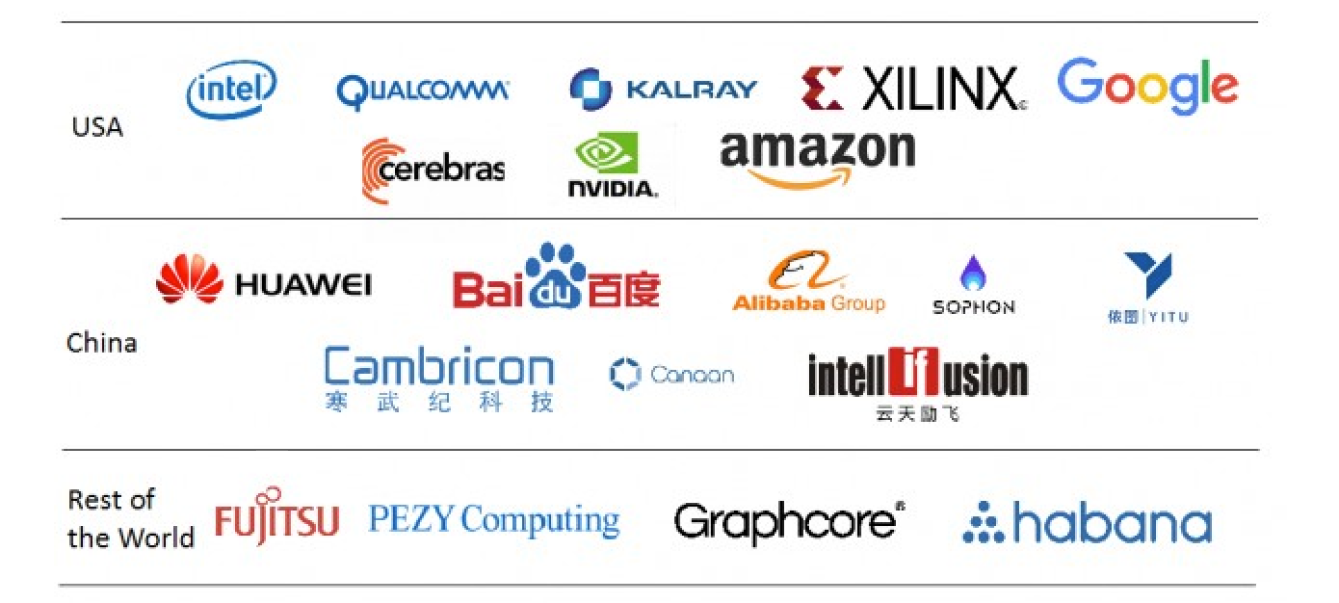
\includegraphics[width=0.5\textwidth]{./figures/Empreses.png}
    \caption{Les capes que te la IA per funcionar}
\end{figure}

\textbf{\Large GPUs}\label{GPUs}\\
Segons Microsoft\cite{Microsoft} una GPUs és:\\
  {\color{gray} La unitat de processament de gràfics (GPU) d'un dispositiu Windows controla el treball relacionat amb els gràfics. Les GPU també es coneixen com a targetes de vídeo o targetes gràfiques.\\
  El treball relacionat amb els gràfics que manegen les GPU inclou els següents elements:
  \begin{itemize}
   \item El grafisme
   \item Efectes
   \item Video
   \item Videojocs
  \end{itemize}
  Hi ha dos tipus bàsics de GPU: GPU integrada i GPU discreta. Coneix els diferents tipus de GPU i troba el que s'ajusta a les teves necessitats:

  \textbf{GPU integrada}
  \begin{itemize}
   \item Les GPU integrades estan integrades directament en el processador principal (CPU).
   \item Les GPU integrades normalment no són tan potents com les GPU discretes, però són més eficients energèticament.
   \item Les GPU integrades sovint són menys costoses que les GPU discretes.
   \item Les GPU integrades permeten que els portàtils siguin més prims, lleugers i eficients.
   \item Les GPU Integrades són excel·lents per a alguns jocs, edició de vídeo lleuger o per treballar amb fotos.
  \end{itemize}

  \textbf{GPU discreta}
  \begin{itemize}
   \item Les GPU discretes són més grans que les GPU integrades i utilitzen més potència, però són les més adequades per a tasques de processament intensiu, com ara edició intensa de fotos i vídeos, treball de disseny i jocs.
   \item En els ordinadors, les GPU discretes són una targeta independent de la CPU, i que es troba en la seva pròpia targeta, fora de la CPU.
   \item Els ordinadors portàtils i tauletes també poden tenir GPU discrets directament a la placa base, però sovint s'afegeixen a la GPU incorporada. La GPU integrada s'utilitza per a tasques gràfiques més lleugeres, mentre que la GPU discreta s'utilitza per a tasques gràfiques més pesades. El canvi entre GPUs a partir de la tasca que es fa permet un equilibri entre rendiment i eficiència energètica.
  \end{itemize}
   }
